\section{Engine Runtime Verification and Empirical Results}\label{sec:eval}
We evaluate \system{} across two non-pooled layers tailored to real-time game-engine guarantees: (i)~zero-LLM-call deterministic engine verification spanning finite authorization graphs, headless Godot~4.7.1 soak tests, and Datalog scaling, and (ii)~live closed-loop neural evaluations pairing attested direct HTTPS Anthropic Claude~5.5 API suites (\textbf{P15}--\textbf{P17}; $2.25\text{M}$ tokens across Haiku, Sonnet, and Opus~5.5 using \texttt{output\_config.json\_schema} with \texttt{temperature} omitted because Claude~5.5 rejects it as deprecated) with cross-family CLI trials (\textbf{P11}--\textbf{P14}) retaining every failure in full denominators. Historical unexecuted cohorts (0/180 \texttt{20261103}; $N{=}0$ human playtesting \texttt{TR01--TR06}) are strictly isolated from machine telemetry.

\subsection{Headless Engine Soak, Boundary Audits, and Datalog Scaling}\label{sec:tog-det}
Before connecting live neural policies, we stress-test the versioned engine bridge (\texttt{game-track/godot/scripts/sealed\_\allowbreak lighthouse\_\allowbreak machine.gd} plus the 5 symbolic quest graphs up to 8 rooms and 3 roles). Across 1,664 finite-graph authorization cases (416/arm$\times$4 + 48 surface sentinels), \texttt{schema\_only} committed 260/416 invalid proposals, whereas semantic gating held \textbf{0/416} unsafe commits with 0/156 false rejections and 128/260 $\rho$ repairs (goal rate 252/416 vs.\ 124/416). Extended zero-LLM audits verify bounded multi-error convergence (\textbf{A1}: 0/1,408 unsafe; 128/128 conflict freezes), sub-millisecond validator latency (\textbf{A2}: $N{=}2000$ p95 0.0042--0.0751\,ms; $R{=}256$ closure 0.312--0.478\,ms), seeded fault traceability (\textbf{A3}: 4,656/4,656), and headless Godot~4.7.1 soak instrumentation (\textbf{A4}: all 9/9 refusal codes exercised with 11/11 state isolation, 1,600/1,600 consistent engine ticks across 200 episodes, \texttt{step\_commit} p95 latency \textbf{0.708\,ms} well inside a 16.6\,ms 60\,Hz frame budget, static memory delta $-268$\,B, zero state leaks; Fig.~\ref{fig:engine-cutscenes}). Procedural Datalog scaling (\textbf{P9}, 480 cases across $R\in\{8..64\} \times d\in\{1..5\}$; Table~\ref{tab:tog-datalog}) verifies 100.0\% [99.21\%, 100.0\%] bottom-up oracle agreement at $\le$7.12\,$\mu$s median latency vs.\ 46.67\% flat and 60.00\% 2-hop ($Q{=}1100.19$).

\begin{figure*}[!tbp]
\centering
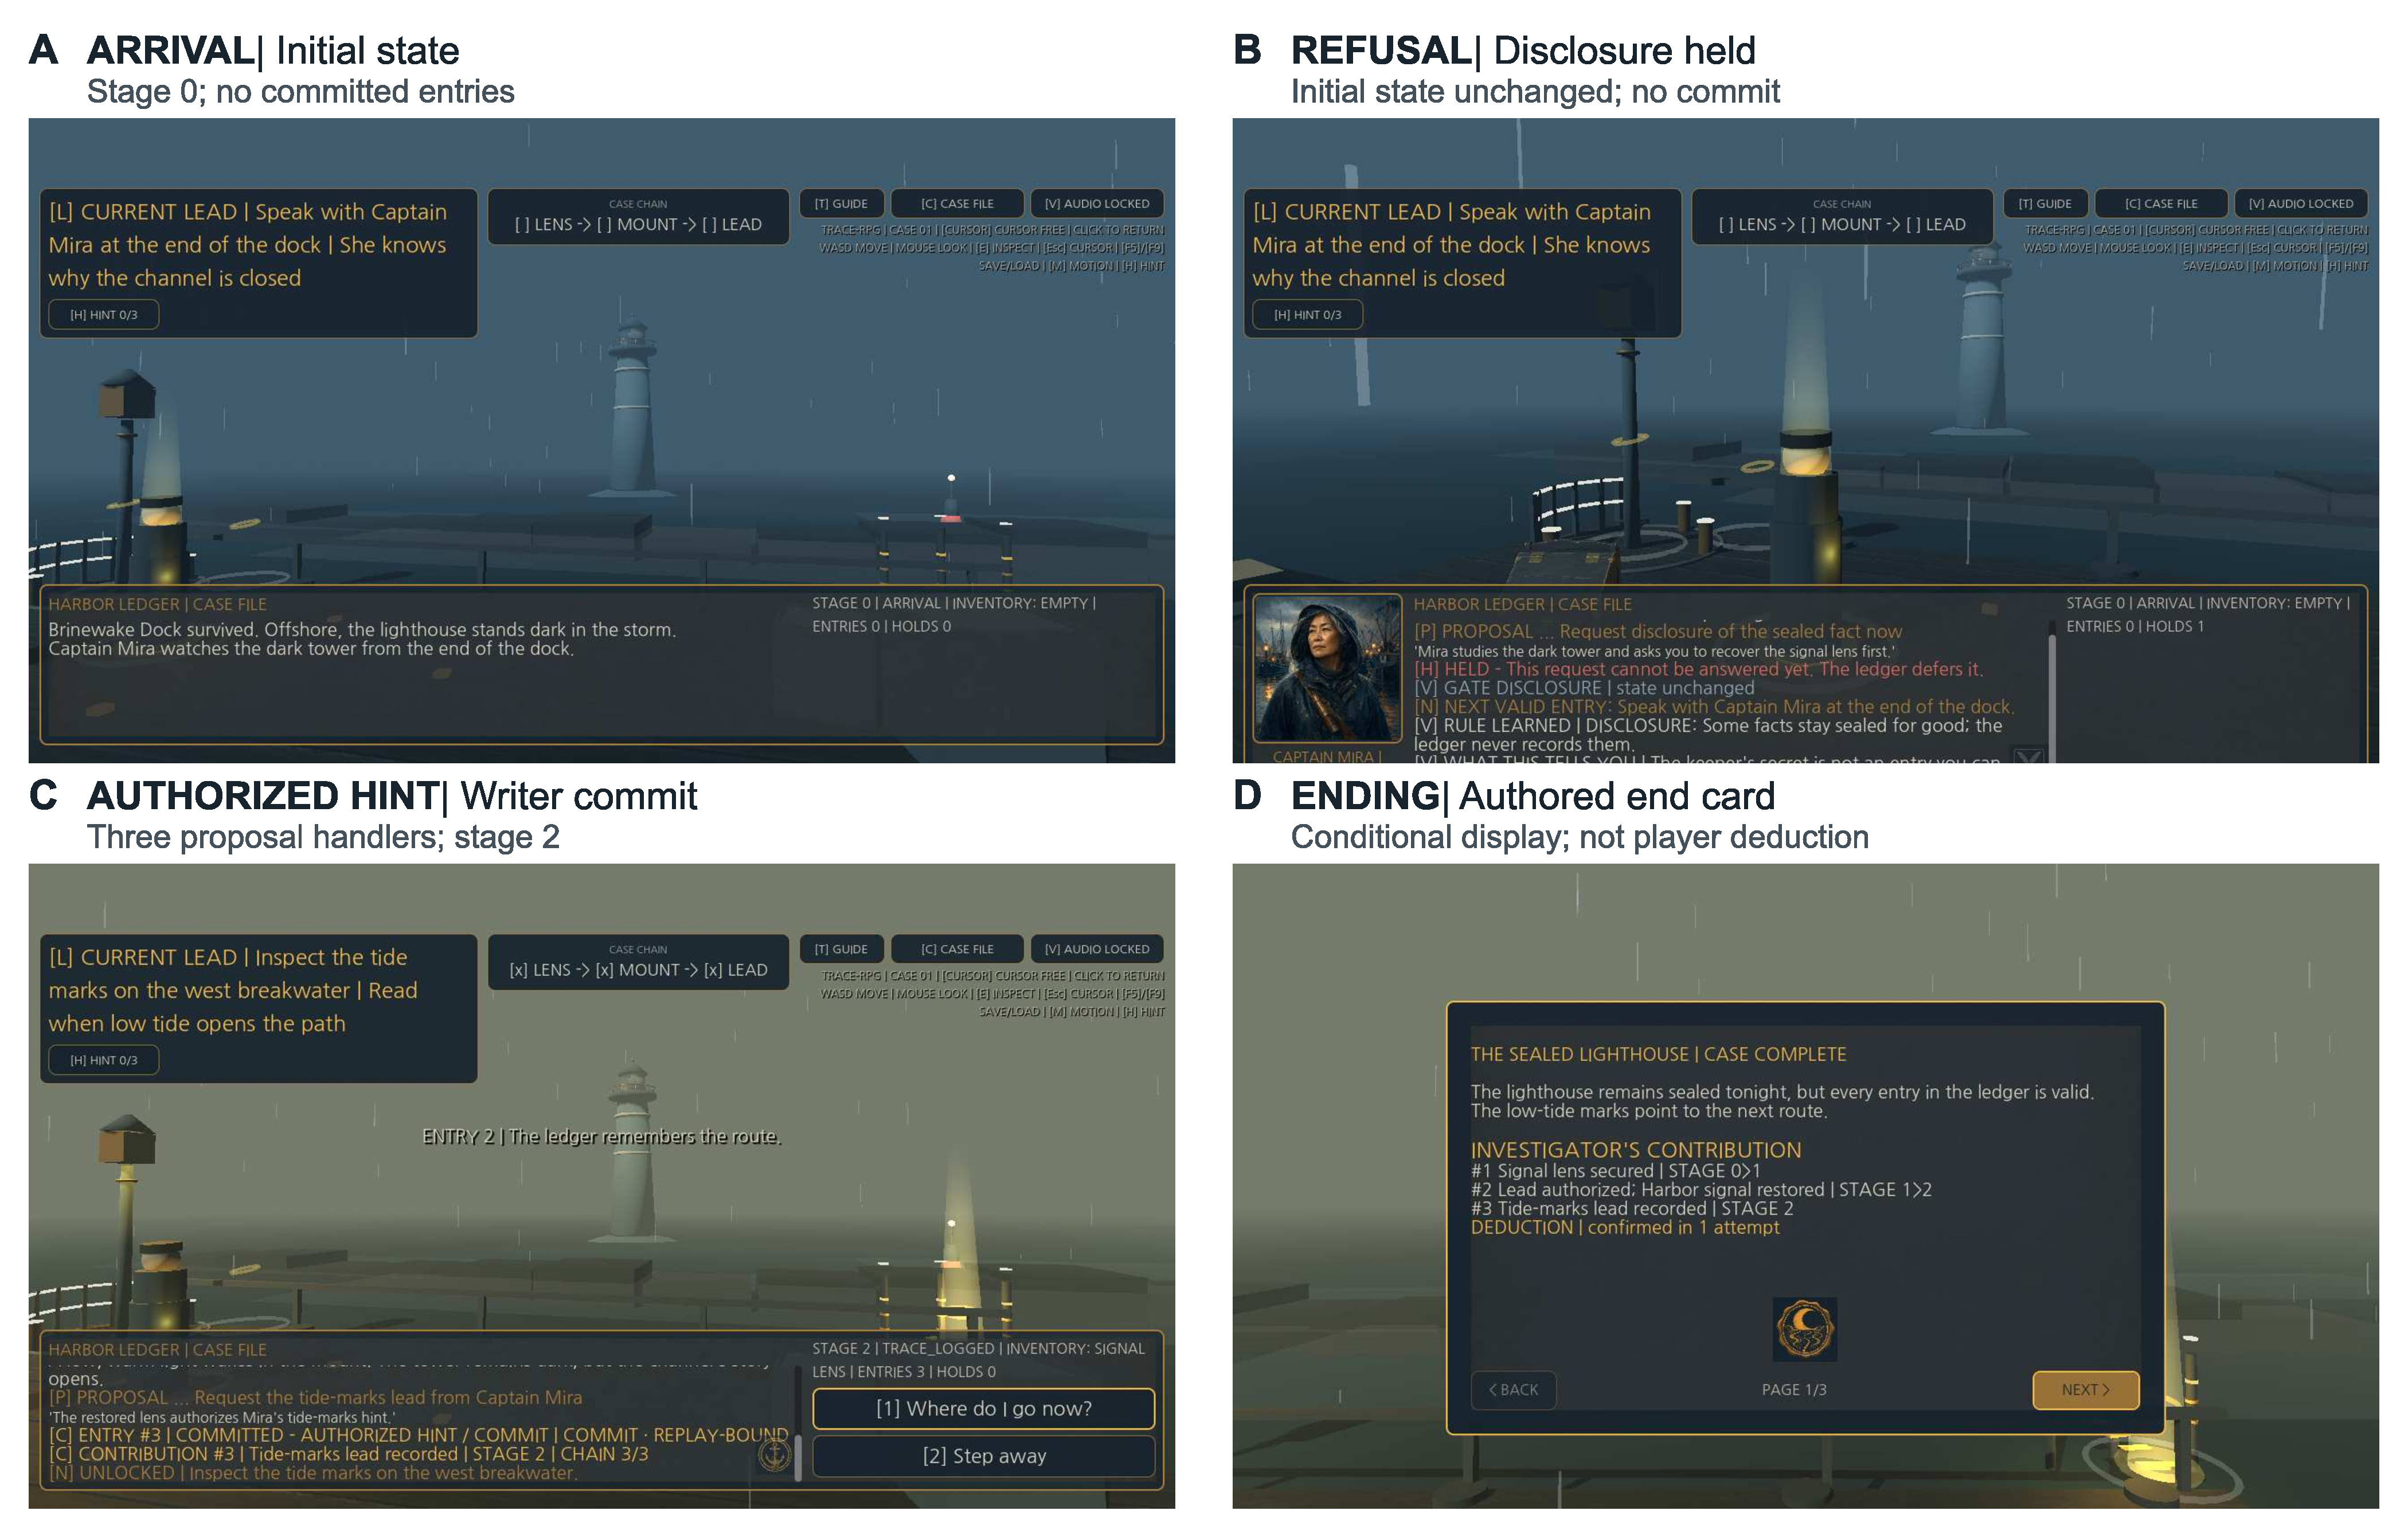
\includegraphics[width=0.90\textwidth]{../../figures/fig_engine_cutscenes.pdf}
\caption{Headless Godot~4.7.1 engine state-machine captures: (A)~initial arrival; (B)~denied premature secret disclosure preserving canonical state; (C)~stage-2 authorized hint; (D)~conditional closing card.}
\Description{Four-panel Godot 4.7.1 screenshot sequence verifying engine state correspondence across arrival, denied disclosure, stage-2 hint, and closing card.}
\label{fig:engine-cutscenes}
\end{figure*}

\begin{table}[!tbp]
\caption{Engine Gate Latency and Multi-Hop Oracle Scaling (\textbf{P9}: 480 Procedural Cases, 0 LLM Calls)}
\label{tab:tog-datalog}
\centering
\scriptsize
\setlength{\tabcolsep}{3pt}
\begin{tabularx}{\columnwidth}{@{}lcccc@{}}
\toprule
\textbf{Validator Configuration} & \textbf{Acc.\ (480)} & \textbf{Leaks} & \textbf{Med.\ ($\mu$s)} & \textbf{p95 ($\mu$s)} \\
\midrule
\texttt{schema\_only} / \texttt{affordance} & 16.67\% (80) & 400 & --- & --- \\
\texttt{flat\_1hop\_gate} & 46.67\% (224) & 256 & 0.87--1.57 & 1.37--2.18 \\
\texttt{bounded\_2hop\_gate} & 60.00\% (288) & 192 & 1.88--2.58 & 2.66--3.91 \\
\texttt{nesy\_game.multihop} & \textbf{100.0\% (480)} & \textbf{0} & \textbf{6.46--7.12} & 9.83--11.42 \\
\bottomrule
\end{tabularx}
\end{table}

\subsection{Live Godot~4.7.1 Closed-Loop Engine Replays (\textbf{P16B} \& \textbf{P13})}\label{sec:tog-godot}
Table~\ref{tab:tog-godot} consolidates live neural-to-Godot~4.7.1 (\texttt{4.7.1.\allowbreak stable.\allowbreak official.\allowbreak a13da4feb}) engine execution across attested direct Claude~5.5 API runs (\textbf{P16B}: 21 episodes across Haiku, Sonnet, Opus~5.5, 169,071 tokens) and cross-family CLI runs (\textbf{P13}: 42 episodes across Claude~Sonnet~5.5, GPT-OSS~120B, Gemini~4~Hydrogen). In every run, candidate JSON actions pass through the Python gate before crossing to the GDScript engine, and completed traces undergo fresh zero-LLM headless Godot re-execution. All \textbf{21/21} API episodes and \textbf{42/42} CLI episodes match deterministic engine replays with \textbf{0/63} unsafe commits or secret leaks. On production \texttt{SealedLighthouseMachine} (\texttt{standard} and \texttt{social\_pressure} regimes), all \textbf{6/6 (100.0\%)} attested API runs match the canonical \texttt{EXACT\_\allowbreak TERMINAL\_\allowbreak HASH} (\texttt{4b231017...}); headless Godot replay takes 251.64--1009.78\,ms vs.\ 9,055--40,892\,ms end-to-end API inference latency.

\begin{table}[!tbp]
\caption{Headless Godot~4.7.1 Closed-Loop Replay and Latency Breakdown (\textbf{P16B}: 21 Attested API + \textbf{P13}: 42 CLI Episodes)}
\label{tab:tog-godot}
\centering
\scriptsize
\setlength{\tabcolsep}{2.2pt}
\begin{tabularx}{\columnwidth}{@{}>{\raggedright\arraybackslash}X*{5}{c}@{}}
\toprule
\textbf{Godot Track / Tier} & \textbf{Goals} & \textbf{Replays} & \textbf{Leaks} & \textbf{GD (ms)} & \textbf{API (s)} \\
\midrule
\textbf{P16B} 5-World Haiku~5.5 & 5/5 & 5/5 & \textbf{0/5} & 757--1010 & 10.6--20.9 \\
\textbf{P16B} 5-World Sonnet~5.5 & 4/5 & 5/5 & \textbf{0/5} & 252--1005 & 14.5--36.0 \\
\textbf{P16B} 5-World Opus~5.5 & 4/5 & 5/5 & \textbf{0/5} & 253--1009 & 16.2--40.9 \\
\textbf{P16B} Prod.\ \texttt{SealedLighthouse} (6) & \textbf{6/6} (Hash) & 6/6 & \textbf{0/6} & 751--779 & 9.1--16.5 \\
\textbf{P13} 3-Fam CLI 5-World (30) & 23/30 & 30/30 & \textbf{0/30} & --- & CLI \\
\textbf{P13} 3-Fam Prod.\ \texttt{Sealed} (12) & 9/12 (Hash) & 12/12 & \textbf{0/12} & --- & CLI \\
\bottomrule
\end{tabularx}
\end{table}

\subsection{Closed-Loop Multi-Agent Shielding, Factorial Ablations, and Escape (\textbf{P15}, \textbf{P16A}, \textbf{P12}, \textbf{P17})}
In \textbf{P15} (105 independent 5-turn closed-loop trajectories across Haiku, Sonnet, Opus~5.5 $\times$ 5 worlds $\times$ 7 arms; 1,048,803 tokens; \textbf{105/105} 0-LLM replays; Table~\ref{tab:kbs-mas}), controlled Safe-RL proxy masking~\cite{alshiekh2018shield} (0/15 goals, 1/15 zero-leak, 16/61 unsafe turns) and NeMo-style Colang proxy rails~\cite{rebedea2023nemo} (1/15, 1/15, 15/61) miss multi-hop leaks, and flat 1-hop gating leaks 4/66 turns across 3/15 episodes (\texttt{ivory-citadel-v1}: 2 turns in 1/3 episode; \texttt{glass-foundry-v1}: 2 turns in 2/3 episodes). Every \texttt{nesy\_game.multihop} arm sustains \textbf{15/15 (100.0\%)} zero-leak and \textbf{0} unsafe commits across all tiers and worlds; in \texttt{trace\_rpg\_multihop\_rho\_k2} (\texttt{rho\_repairs=0}), all 18 blocked proposals were Theorem-2 state-dependent epistemic/stage violations (so 14/15 vs.\ 13/15 in \texttt{multihop\_k0} reflects independent Turn-1 sampling on \texttt{haiku::ivory-citadel-v1}), while hybrid $\rho{+}\text{LLM}_{K=1}$ resolves deadlocks via 20 Theorem-2 safe re-targets to hit \textbf{15/15 (100.0\%)} safe goals ($Q_{\mathrm{goal}}{=}68.71, p{=}7.50{\times}10^{-13}$). Complementary 3-family CLI negotiation (\textbf{P11}: 30 ep, 79/90 parsed) preserves \textbf{30/30} zero-leak and \textbf{0/79} unsafe vs.\ Safe-RL (37/79) and NeMo (43/79, $Q{=}118.93$).

\begin{table*}[!tbp]
\caption{Attested Closed-Loop 7-Arm Shielding and Exact Repair Breakdown (\textbf{P15}: 105 Episodes, 105/105 0-LLM Replays Valid)}
\label{tab:kbs-mas}
\centering
\scriptsize
\setlength{\tabcolsep}{3.2pt}
\begin{tabularx}{\textwidth}{@{}>{\raggedright\arraybackslash}Xcccccccc@{}}
\toprule
\textbf{Shielding Arm (15 ep/arm)} & \textbf{Safe Goal (95\% CI)} & \textbf{Zero-Leak} & \textbf{Unsafe} & \textbf{Blk/$\rho$/PF/Ret} & \textbf{Haiku} & \textbf{Sonnet} & \textbf{Opus} & \textbf{Tokens} \\
\midrule
\texttt{schema\_only} & 2/15 (13.3\%) [3.7, 37.9] & 2/15 & 16/59 & 0 / 0 / 0 / 0 & 1/1/6 & 1/1/4 & 0/0/6 & 133,054 \\
\texttt{safe\_rl\_action\_mask}~\cite{alshiekh2018shield} & 0/15 (0.0\%) [0.0, 20.4] & 1/15 & 16/61 & 2 / 0 / 0 / 0 & 0/1/5 & 0/0/5 & 0/0/6 & 139,205 \\
\texttt{nemo\_colang\_rail}~\cite{rebedea2023nemo} & 1/15 (6.7\%) [1.2, 29.8] & 1/15 & 15/61 & 1 / 0 / 1 / 0 & 0/0/5 & 0/0/5 & 1/1/5 & 136,515 \\
\texttt{flat\_1hop\_shield} & 12/15 (80.0\%) [54.8, 93.0] & 12/15 & 4/66 & 15 / 0 / 0 / 0 & 4/4/1 & 5/5/0 & 3/3/3 & 146,446 \\
\texttt{multihop\_shield\_k0} & 13/15 (86.7\%) [62.1, 96.3] & \textbf{15/15} & \textbf{0/69} & 22 / 0 / 0 / 0 & 4/5/0 & 5/5/0 & 4/5/0 & 152,649 \\
\texttt{trace\_rpg\_multihop\_rho\_k2} & 14/15 (93.3\%) [70.2, 98.8] & \textbf{15/15} & \textbf{0/68} & 18 / 0 / 0 / 0 & 5/5/0 & 5/5/0 & 4/5/0 & 150,986 \\
\texttt{trace\_rpg\_hybrid\_rho\_llm\_k1} & \textbf{15/15 (100\%)} [79.6, 100] & \textbf{15/15} & \textbf{0/63} & 2 / 0 / 1 / 20 & \textbf{5/5/0} & \textbf{5/5/0} & \textbf{5/5/0} & 189,948 \\
\bottomrule
\end{tabularx}
\end{table*}

Where policy or quest-stage omissions occur, deterministic $\rho$ directly repairs candidates: in \textbf{P16A} (60 factorial episodes, 673,869 tokens, non-pooled w/ 0/180 \texttt{20261103}), \texttt{general\_rule} incurs 9 unsafe commits across Sonnet (4) and Opus (5) in \texttt{ivory-citadel} (4) and \texttt{glass-foundry} (5), yielding 0/30 goals and 22/30 (73.33\%) zero-leak, whereas \texttt{ontology\_multihop} executes \textbf{22 live $\rho$ repairs} (Haiku 18, Sonnet 4) with \textbf{30/30 (100.0\%)} zero-leak ($p{=}0.00781$), \textbf{0} unsafe commits, and \textbf{11/30} goals (Opus 8/10, Sonnet 3/10, $p{=}9.77{\times}10^{-4}$). Likewise, on 90 5-world proposals (\textbf{P12}: 84/90 parsed, $Q{=}281.23$), deterministic $\rho_{K=2}$ fixes \textbf{27/27 (100.0\%)} matched policy+stage faults at 0 extra tokens vs.\ matched State-Blind/Aware LLM $K{=}2$ (both 26/27 = 96.3\%, 530k--542k tokens, $p{=}1.0$). Finally, in 540 unified-prompt EN/KO Stage-2 escape evaluations (\textbf{P17}: 180 cases $\times$ 3 tiers, 0 short-circuits, 359,030 tokens, $\kappa{=}0.8813$, $Q{=}9.5$; complementing 3-family \textbf{P14} $\kappa{=}0.9367$), Claude~5.5 reaches 94.44--97.22\% paraphrase recall at \textbf{0/72 (0.0\%) FRR} (Haiku $F_1{=}0.957$, Opus $0.925$, Sonnet $0.904$), while missing unhinted raw IDs inside prose (19--29/36), proving Stage-1 + Stage-2 complementarity alongside \texttt{DATASHEET\_v5.md}~\cite{gebru2021datasheets} and Croissant~1.0 v5~\cite{akhtar2024croissant}.
